\documentclass[a4paper,12pt]{article}
\usepackage[pdftex]{graphicx}
\usepackage[magyar]{babel}
\usepackage[T1]{fontenc}
\usepackage[utf8]{inputenc}
\usepackage{multirow}
\usepackage{dcolumn}
\newcolumntype{d}[1]{D{.}{\cdot}{#1} }
\usepackage{indentfirst}
\usepackage{amsmath}
\usepackage{t1enc} 
%\usepackage{epsfig}
%\usepackage{epstopdf}
\usepackage{multirow}
\usepackage{float}
\usepackage{wrapfig}
\usepackage{enumerate}
\usepackage{caption}
\usepackage{subcaption}
\usepackage{color}
\usepackage{array}
\usepackage{bbold}
\usepackage{chngpage}
\bibliographystyle{unsrt}
\usepackage[top=4cm ,bottom=4cm ,left=3cm ,right=3cm]{geometry}
%\usepackage{a4wide}
\linespread{1.3}
\usepackage{xcolor}
%\usepackage{hyperref}
%\hypersetup{hidelinks}

\DeclareGraphicsExtensions{.pdf,.eps,.png,.jpg,.mps,.gif}
\addtolength{\hoffset}{-1cm}
\addtolength{\textwidth}{2cm}
\addtolength{\voffset}{-1cm}

\pdfminorversion=5
\pdfobjcompresslevel=2
\newcommand{\celsius}{ ^\circ C } % °C
\newcommand{\megj}[1]{\textit{\small{Megjegyzés: #1}}}
\newenvironment{bfigure}[1]{	\begin{figure}[#1]
			\begin{bf}}
			{\end{bf}
				\end{figure}}
\newcommand{\icaption}[1]{\caption{\textit{\textmd{#1}}}}
\newcommand{\brref}[1]{(\ref{#1}. ábra)}
\newcommand{\sz}[1]{\emph{#1. szakasz}}
\newcommand{\cg}[1]{   {\color{green}  #1 }   }
\newcommand{\vect}[1]{\boldsymbol{#1}}
\newcommand{\dd}{\mathrm{d}}

\begin{document}
	\begin{titlepage}
\author{\\Jakobi Ádám  \\ 
}

\title{\textsc{Számítógépes Szimulációk} \\ 
\huge{\textbf{Harmonikus Oszcillátor}\\
\vspace{10pt}\textsc{JEGYZŐKÖNYV}}}


	
\centering
\maketitle
	\thispagestyle{empty}
\begin{figure}[h!]
\centering

\includegraphics[scale=0.08]{eltelogo.jpg}
\end{figure}
%\vspace{\stretch{1}}
	\end{titlepage}
	
\newpage
%\tableofcontents   %tartalomjegyzék
%\newpage
%%\pagestyle{myheadings}
%\newpage

\section{Bevezető}
Az első beadandó célja harmonikus oszcillátor modellezése, mely a legtöbb valós fizikai jelenséggel ellentétben egzakt módon leírható. Így van lehetőségünk arra, hogy összevessük numerikus módszereink hatékonyságát az analitikus eredménnyel.

A feladatunk az Euler-Cromer algoritmus, az Euler algoritmus és az analitikus megoldás összehasonlítása. Az adatokat egy c++ program segítségével generáltam. A paramétereket parancssori argumentumként adtam meg: szögsebesség, kezdeti kitérés, kezdeti sebesség, periódusok száma, egy periódus alatti lépések száma. A végeredményt egy text file-ba irattam ki, 10 oszlopba. Az első oszlop az eltelt idő, majd 3-3-3 oszlop az Euler-Cromer, Euler és analitikus módszer kitérés, sebesség és energia értékeinek feleltethetők meg. A programot különböző bemeneti paraméterekkel futtattam, a kapott eredményeket lent ábrázolom és diskutálom. Az ábrákat python 3 notebook segítségével készítettem.

\section{Elméleti bevezetés}

\subsection{Harmonikus oszcillátor mozgásegyenletei}

Mozgásegyenlete:
$$m \cdot \dfrac{d^2x}{dt^2}=-m \cdot {\omega}^2 \cdot x$$

Integrálva megkapható a kitérés és a sebesség időfüggvénye (analitikus számolási módszer):
$$x(t) = x_0 \cdot \cos(\omega \cdot t) + (\frac{v_0}{\omega}) \cdot \sin(\omega \cdot t)$$
$$v(t) = -x_0 \cdot \omega \cdot \sin(\omega \cdot t) + v_0 \cdot \cos(\omega \cdot t)$$

\subsection{Numerikus módszerek}

A harmonikus oszcillátor mozgásegyenlete másodrendű, amely átírható két elsőrendű csatolt

egyenletre:
$$\frac{dx}{dt}=v$$
$$\frac{dv}{dt}=-w^2 \cdot x = a$$

\newpage

Euler-módszer:
$$v(t+dt)=v(t) + a(t) \cdot dt$$
$$x(t+dt)=x(t)+v(t) \cdot dt$$

Euler-Cromer-szabály:
$$v(t+dt)=v(t) + a(t) \cdot dt$$
$$x(t+dt)=x(t)+v(t+dt) \cdot dt$$

Az Euler-Cromer-szbály annyival tér el az Euler-algoritmustól, hogy a második egyenletben már a frissített v(t+dt) szerepel az eredeti v(t) helyett. Utóbbi alkalmas az energia megőrzésére, míg az eredeti algoritmus nem.

A rendszerünk pillanatnyi energiáját pedig a következő képlettel tudjuk kiszámítani:

$$E=\frac{1}{2} \cdot m \cdot v^2 + \frac{1}{2} \cdot m \cdot \omega^2$$

\newpage

\section{Kiértékelés}

\subsection{Kitérés-idő}

Az első feladatban a harmonikus oszcillátor kitérésének és sebességének folyamatát vizsgáltuk az idő függvényében.

\begin{figure}[ht!]
\centering
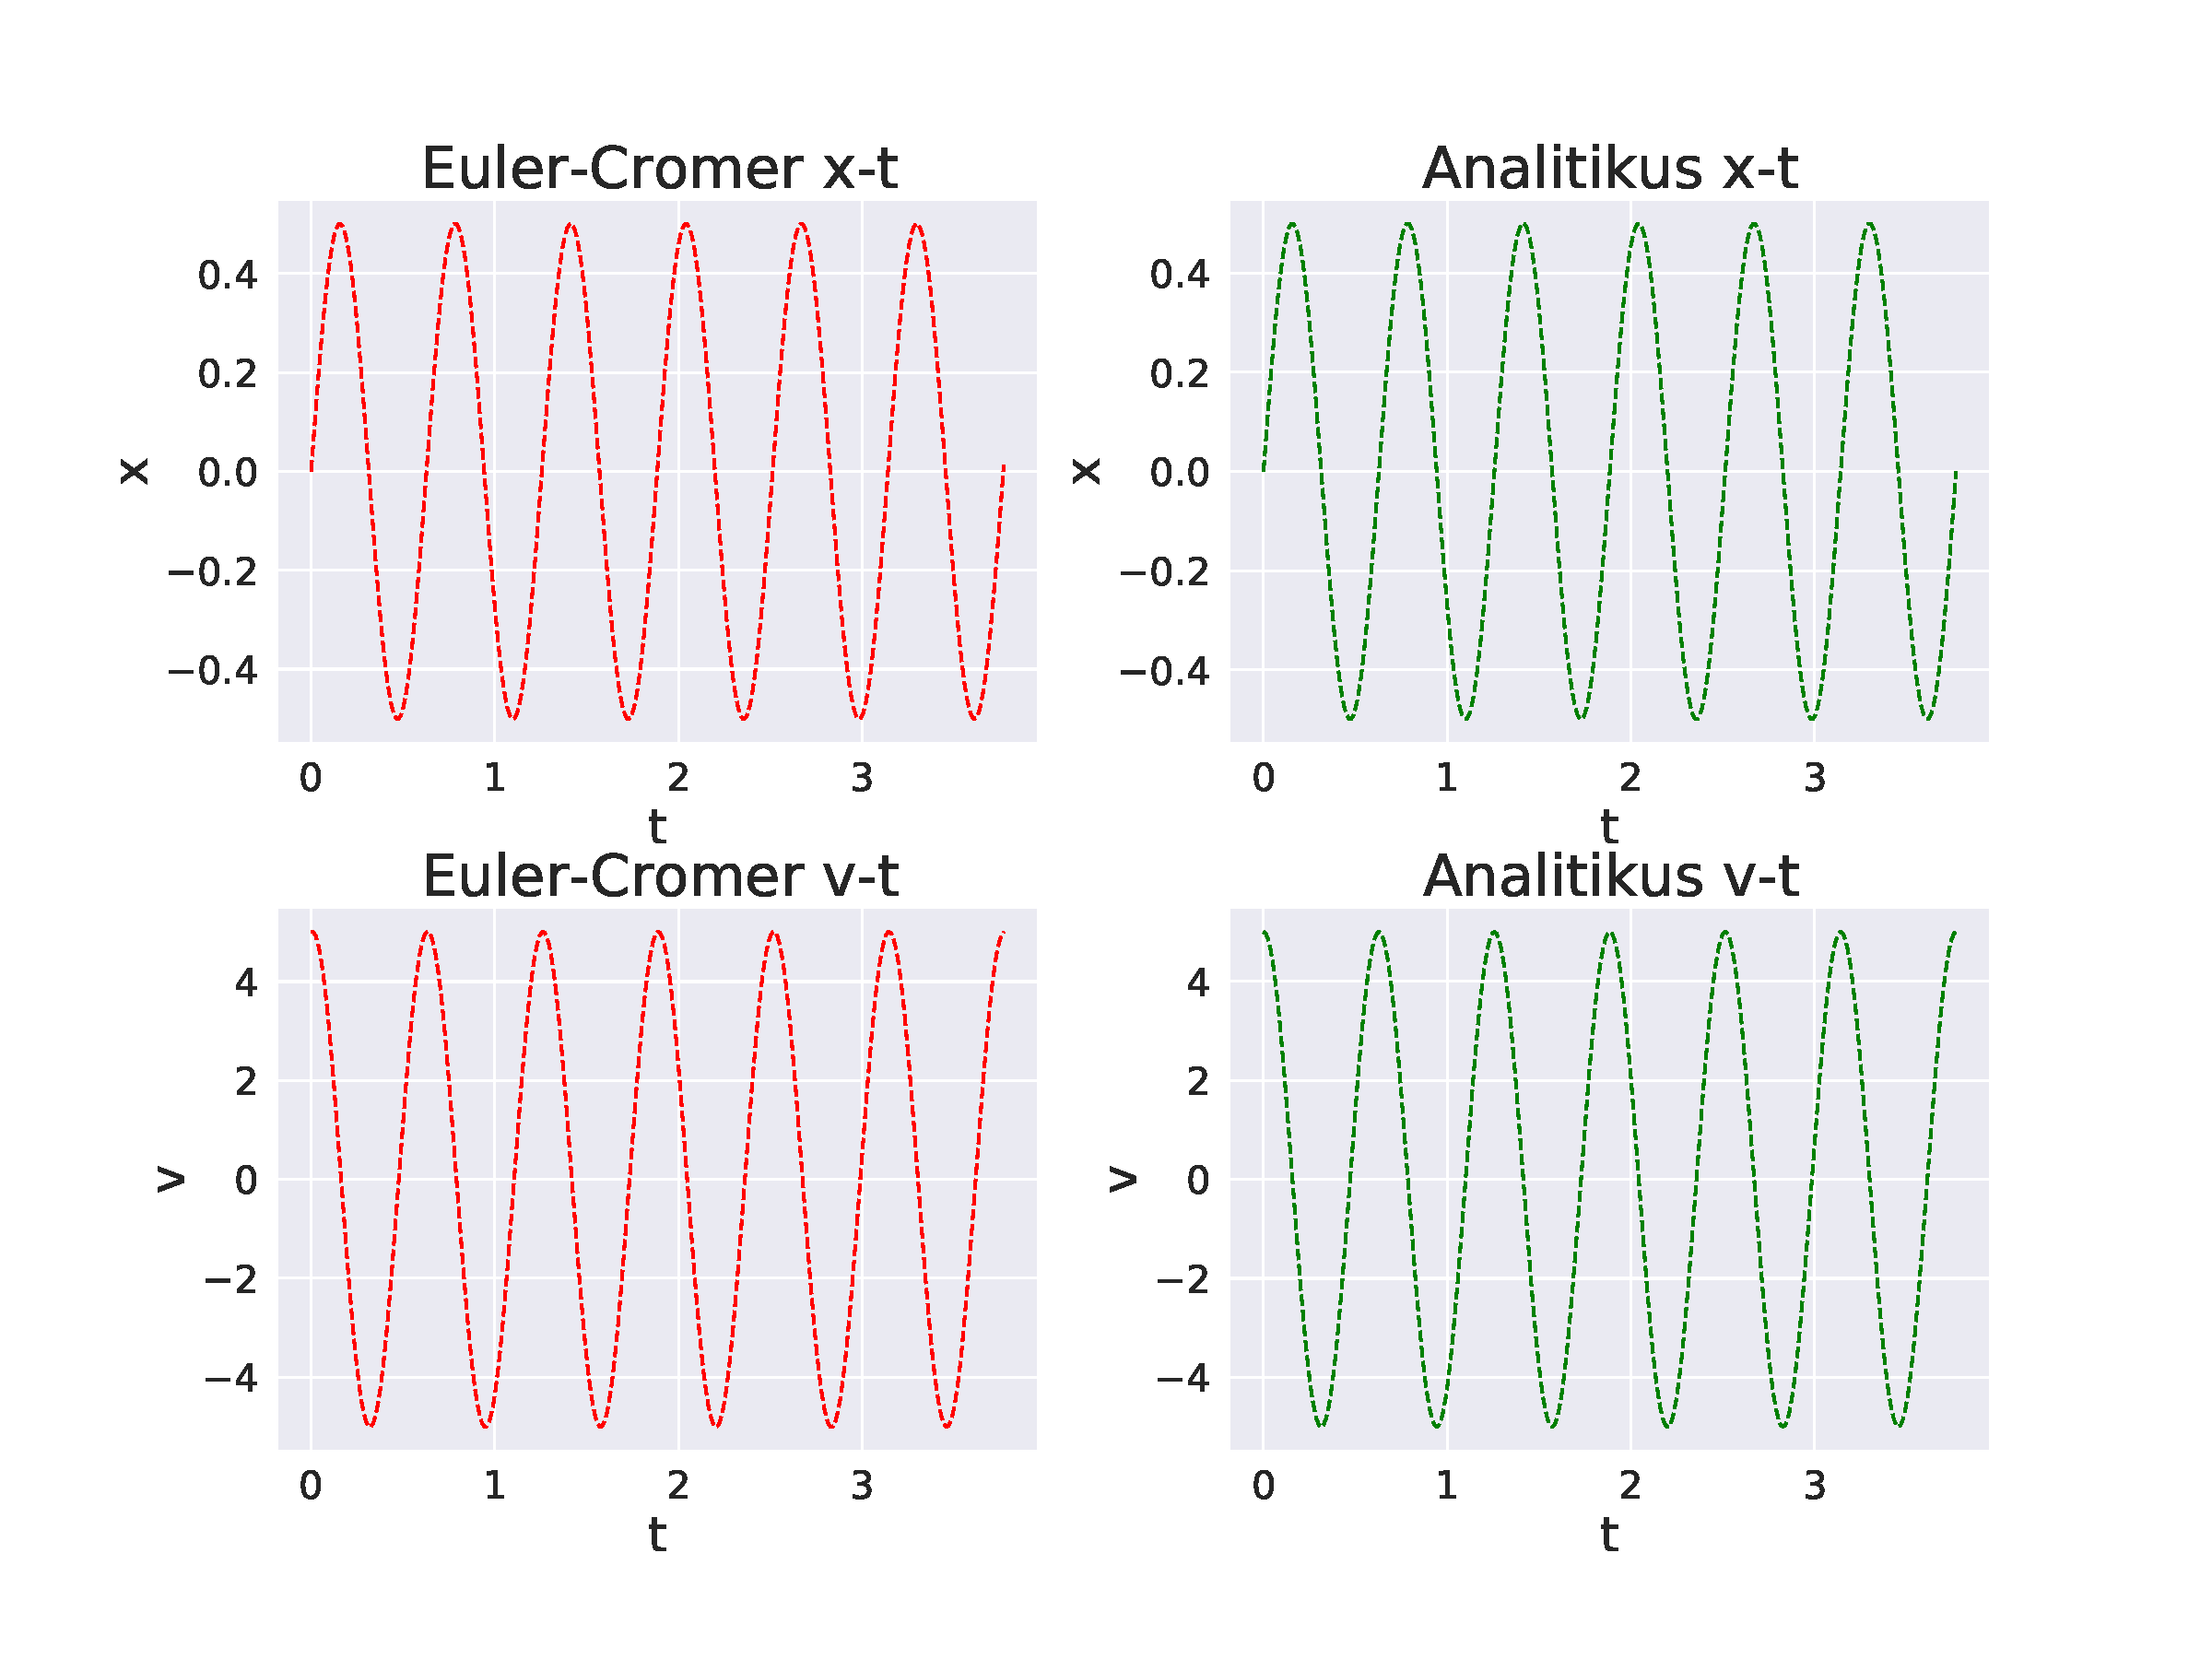
\includegraphics[scale=0.45]{A.pdf}
\caption{Euler-Cromer módszer kitérés-idő grafikonja ($\omega=10$ ; $x_0=0$ ; $v_0=5$ , periódusok száma=6 ; lépésszám periódusonként=50)}
\end{figure}

Az eredményeket az analitikus megoldással összevetve látszik, hogy az elméletből elvártakat kaptuk vissza.

\newpage

\subsection{Fázisdiagram}

A második feladatban a kitérés-sebesség diagramot kellett ábrázolnunk hosszabb időtartamon.

\begin{figure}[ht!]
\centering
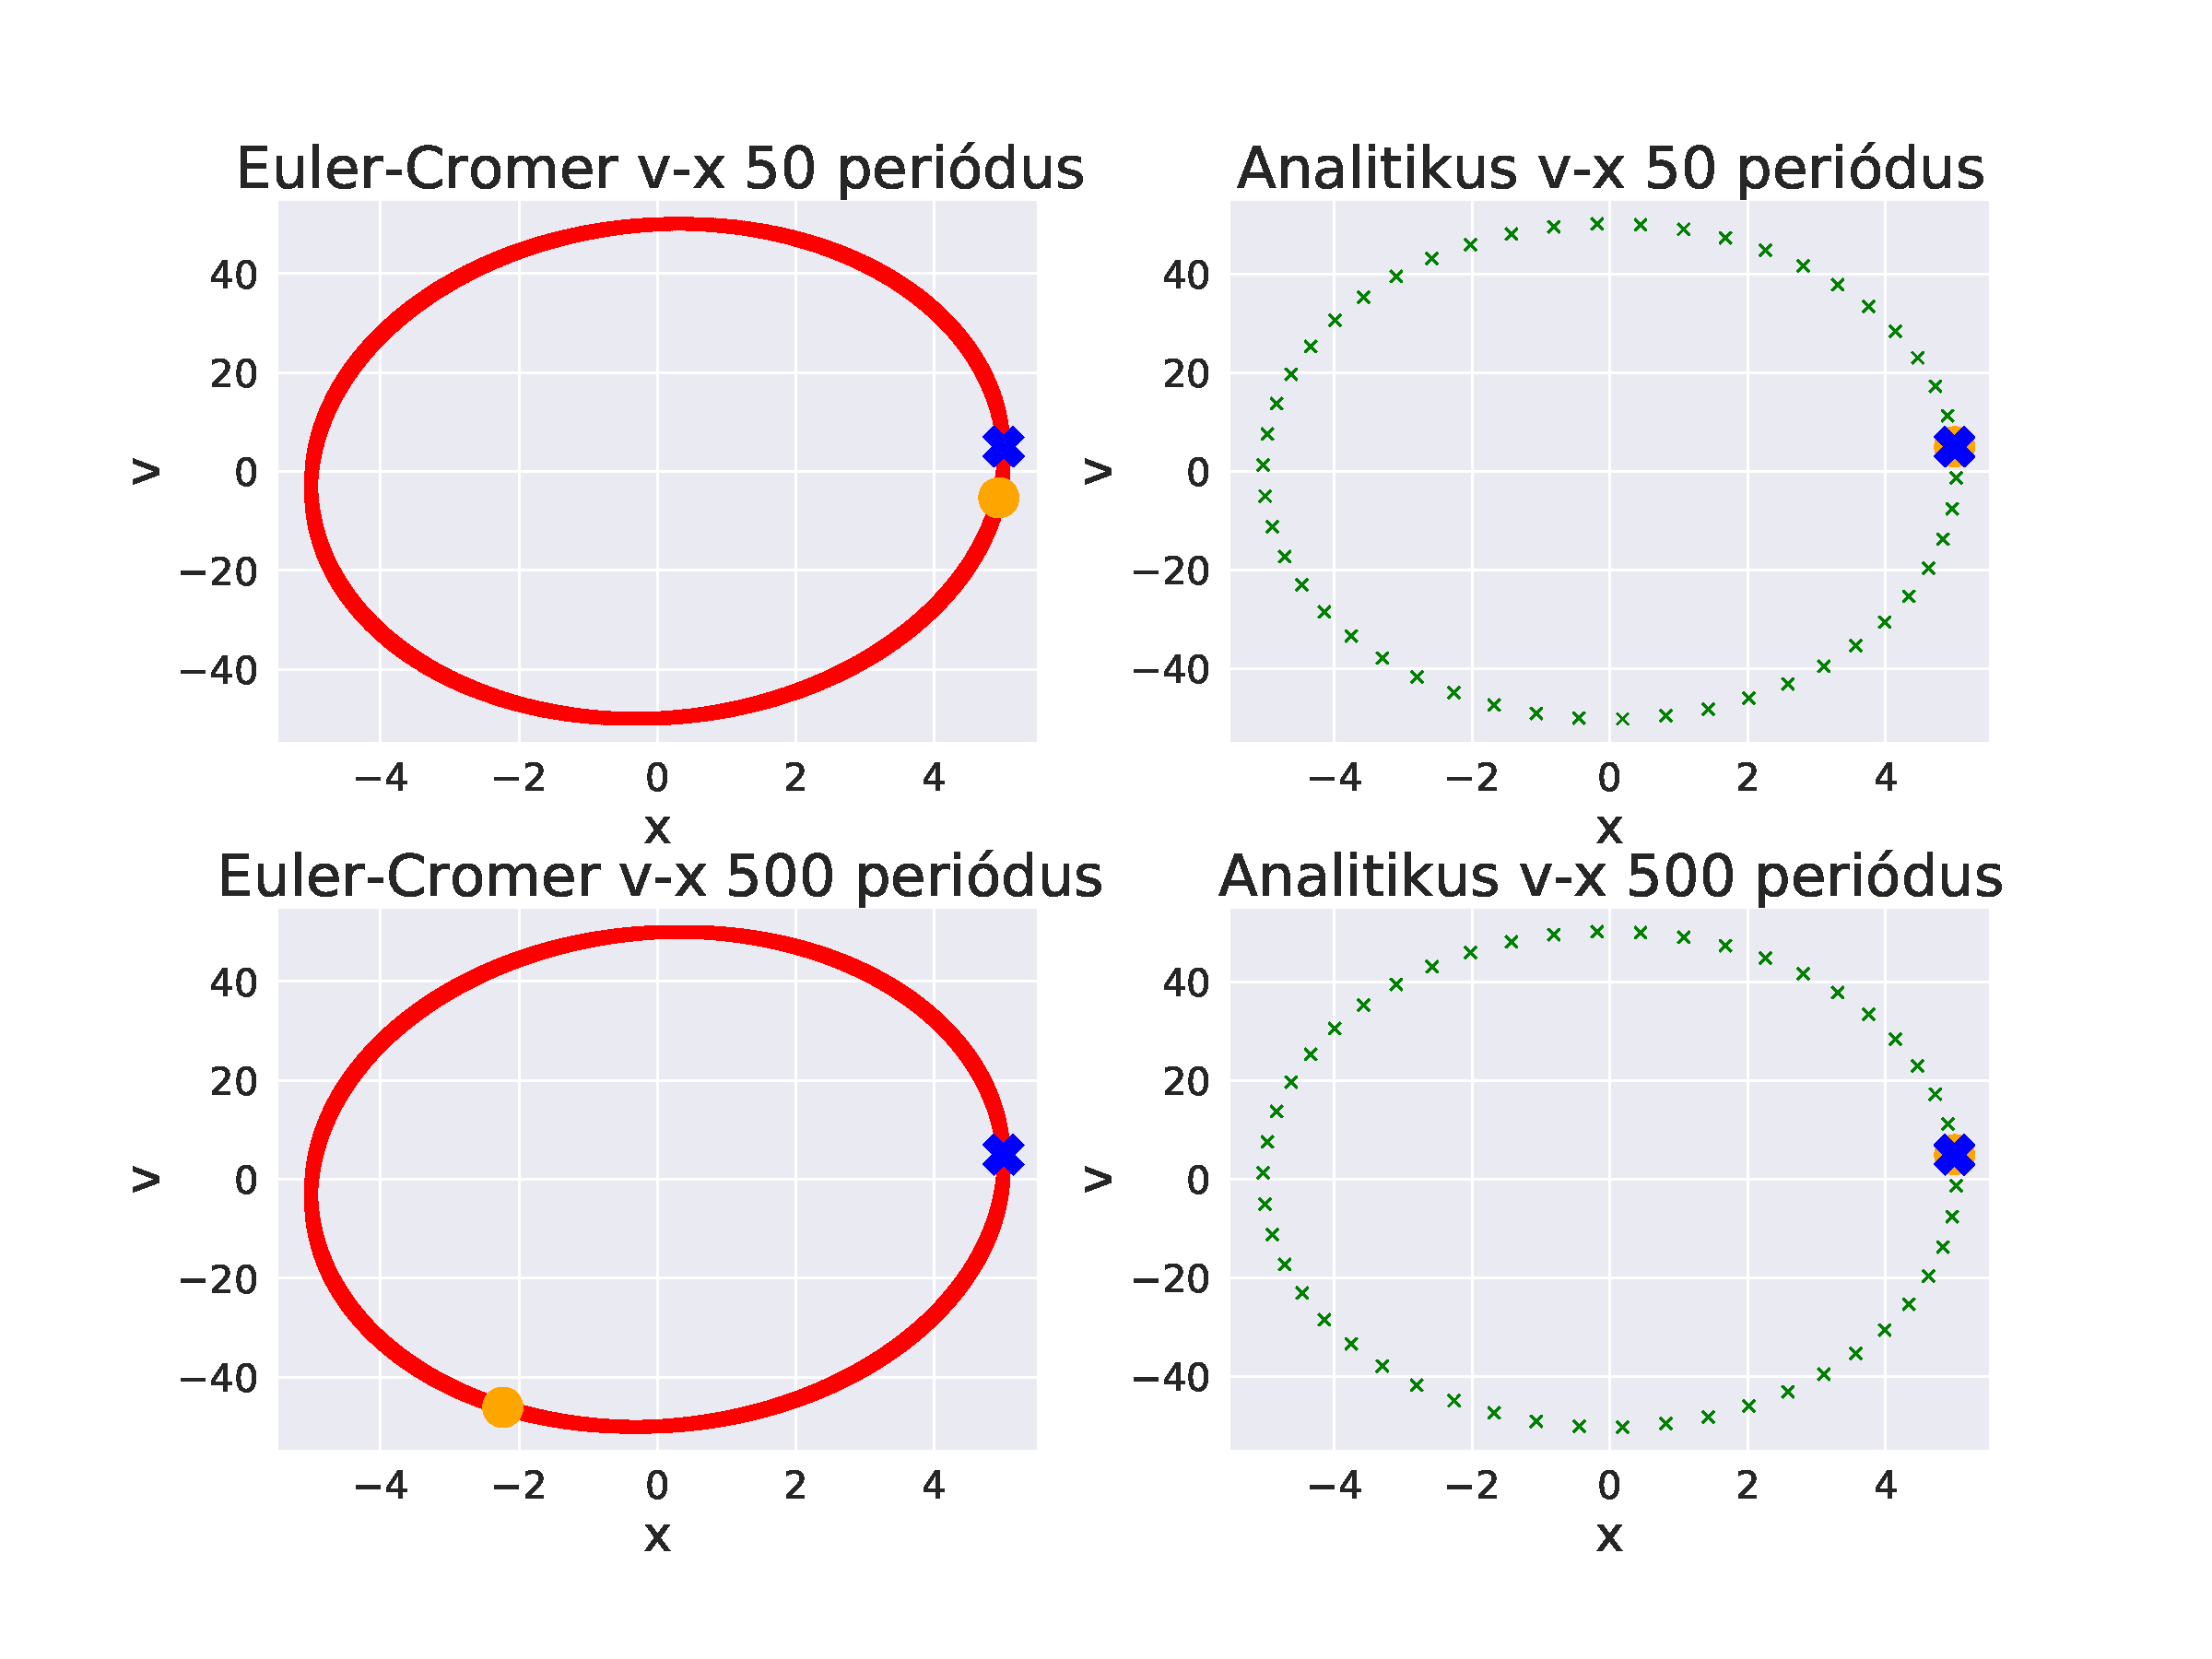
\includegraphics[scale=0.45]{B2.pdf}
\caption{Euler-Cromer módszer fázisdiagramja ($\omega=10$ ; $x_0=5$ ; $v_0=5$ ; lépésszám periódusonként=50)}
\end{figure}

Mint azt az analitikus megoldás is mutatja, azt vártuk, hogy a modellünk tetszőlegesen hosszú futtatásra ellipszis pályát ad, melynek pontjai periódusonként azonos koordinátákon jelennek meg (ez látszik is az analitikus ábrákon).

Ennek ellenére, az Euler-Cromer módszernél a számolt pontok koordinátáiban folyamatos elcsúszás figyelhető meg. Az elcsúszás érzékeltetésére kiemeltem kék X jelölővel az első, és sárga O jelölővel az utolsó számolt pontot, melyeknek az analitikus modell alapján egy pontba kéne esnie. A felső ábra és alsó ábra segít illusztrálni az eltolódás mértékét a ciklusok számának függvényében.

\bigskip

Egy másik probléma is megfigyelhető: ha periódusonként kevés a lépésszám, akkor a fázisdiagram ellipszistengelye elfordul az elmélet szerint várt vízszinteshez képest.

\begin{figure}[ht!]
\centering
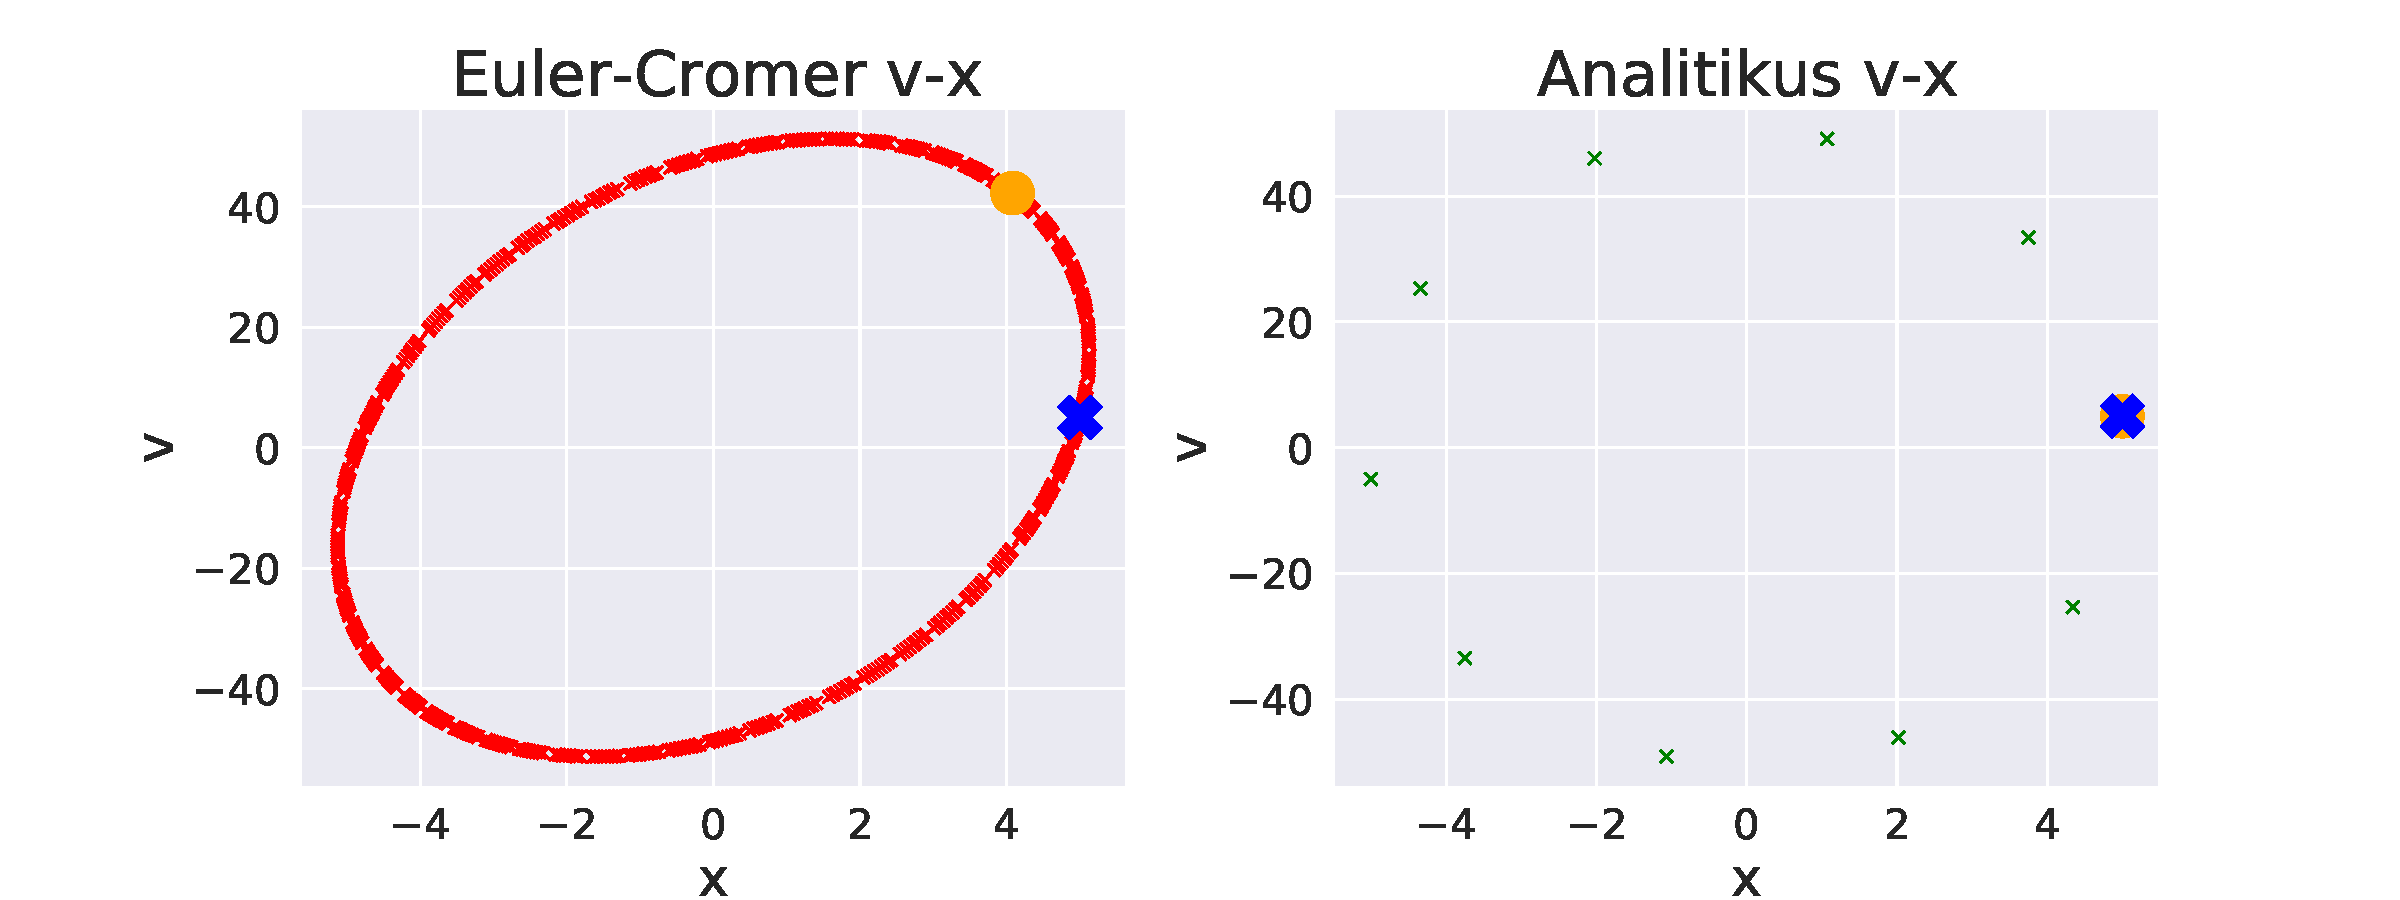
\includegraphics[scale=0.45]{B1.pdf}
\caption{Euler-Cromer módszer elfordult fázisdiagramja ($\omega=10$ ; $x_0=5$ ; $v_0=5$ ; periódusok száma=50 ; lépésszám periódusonként=10)}
\end{figure}

\subsection{Energiamegmaradás}

A harmadik feladatban az Euler és Euler-Cromer algoritmusokat kellett összehasonlítanunk az energiamegmaradás szempontjából.

Az Euler algoritmus energiája folyamatosan nő, melyet a pontatlan léptetés okoz, amely során a kitérések és sebességek maximuma is folyamatosan emelkedik.

\newpage

\begin{figure}[ht!]
\centering
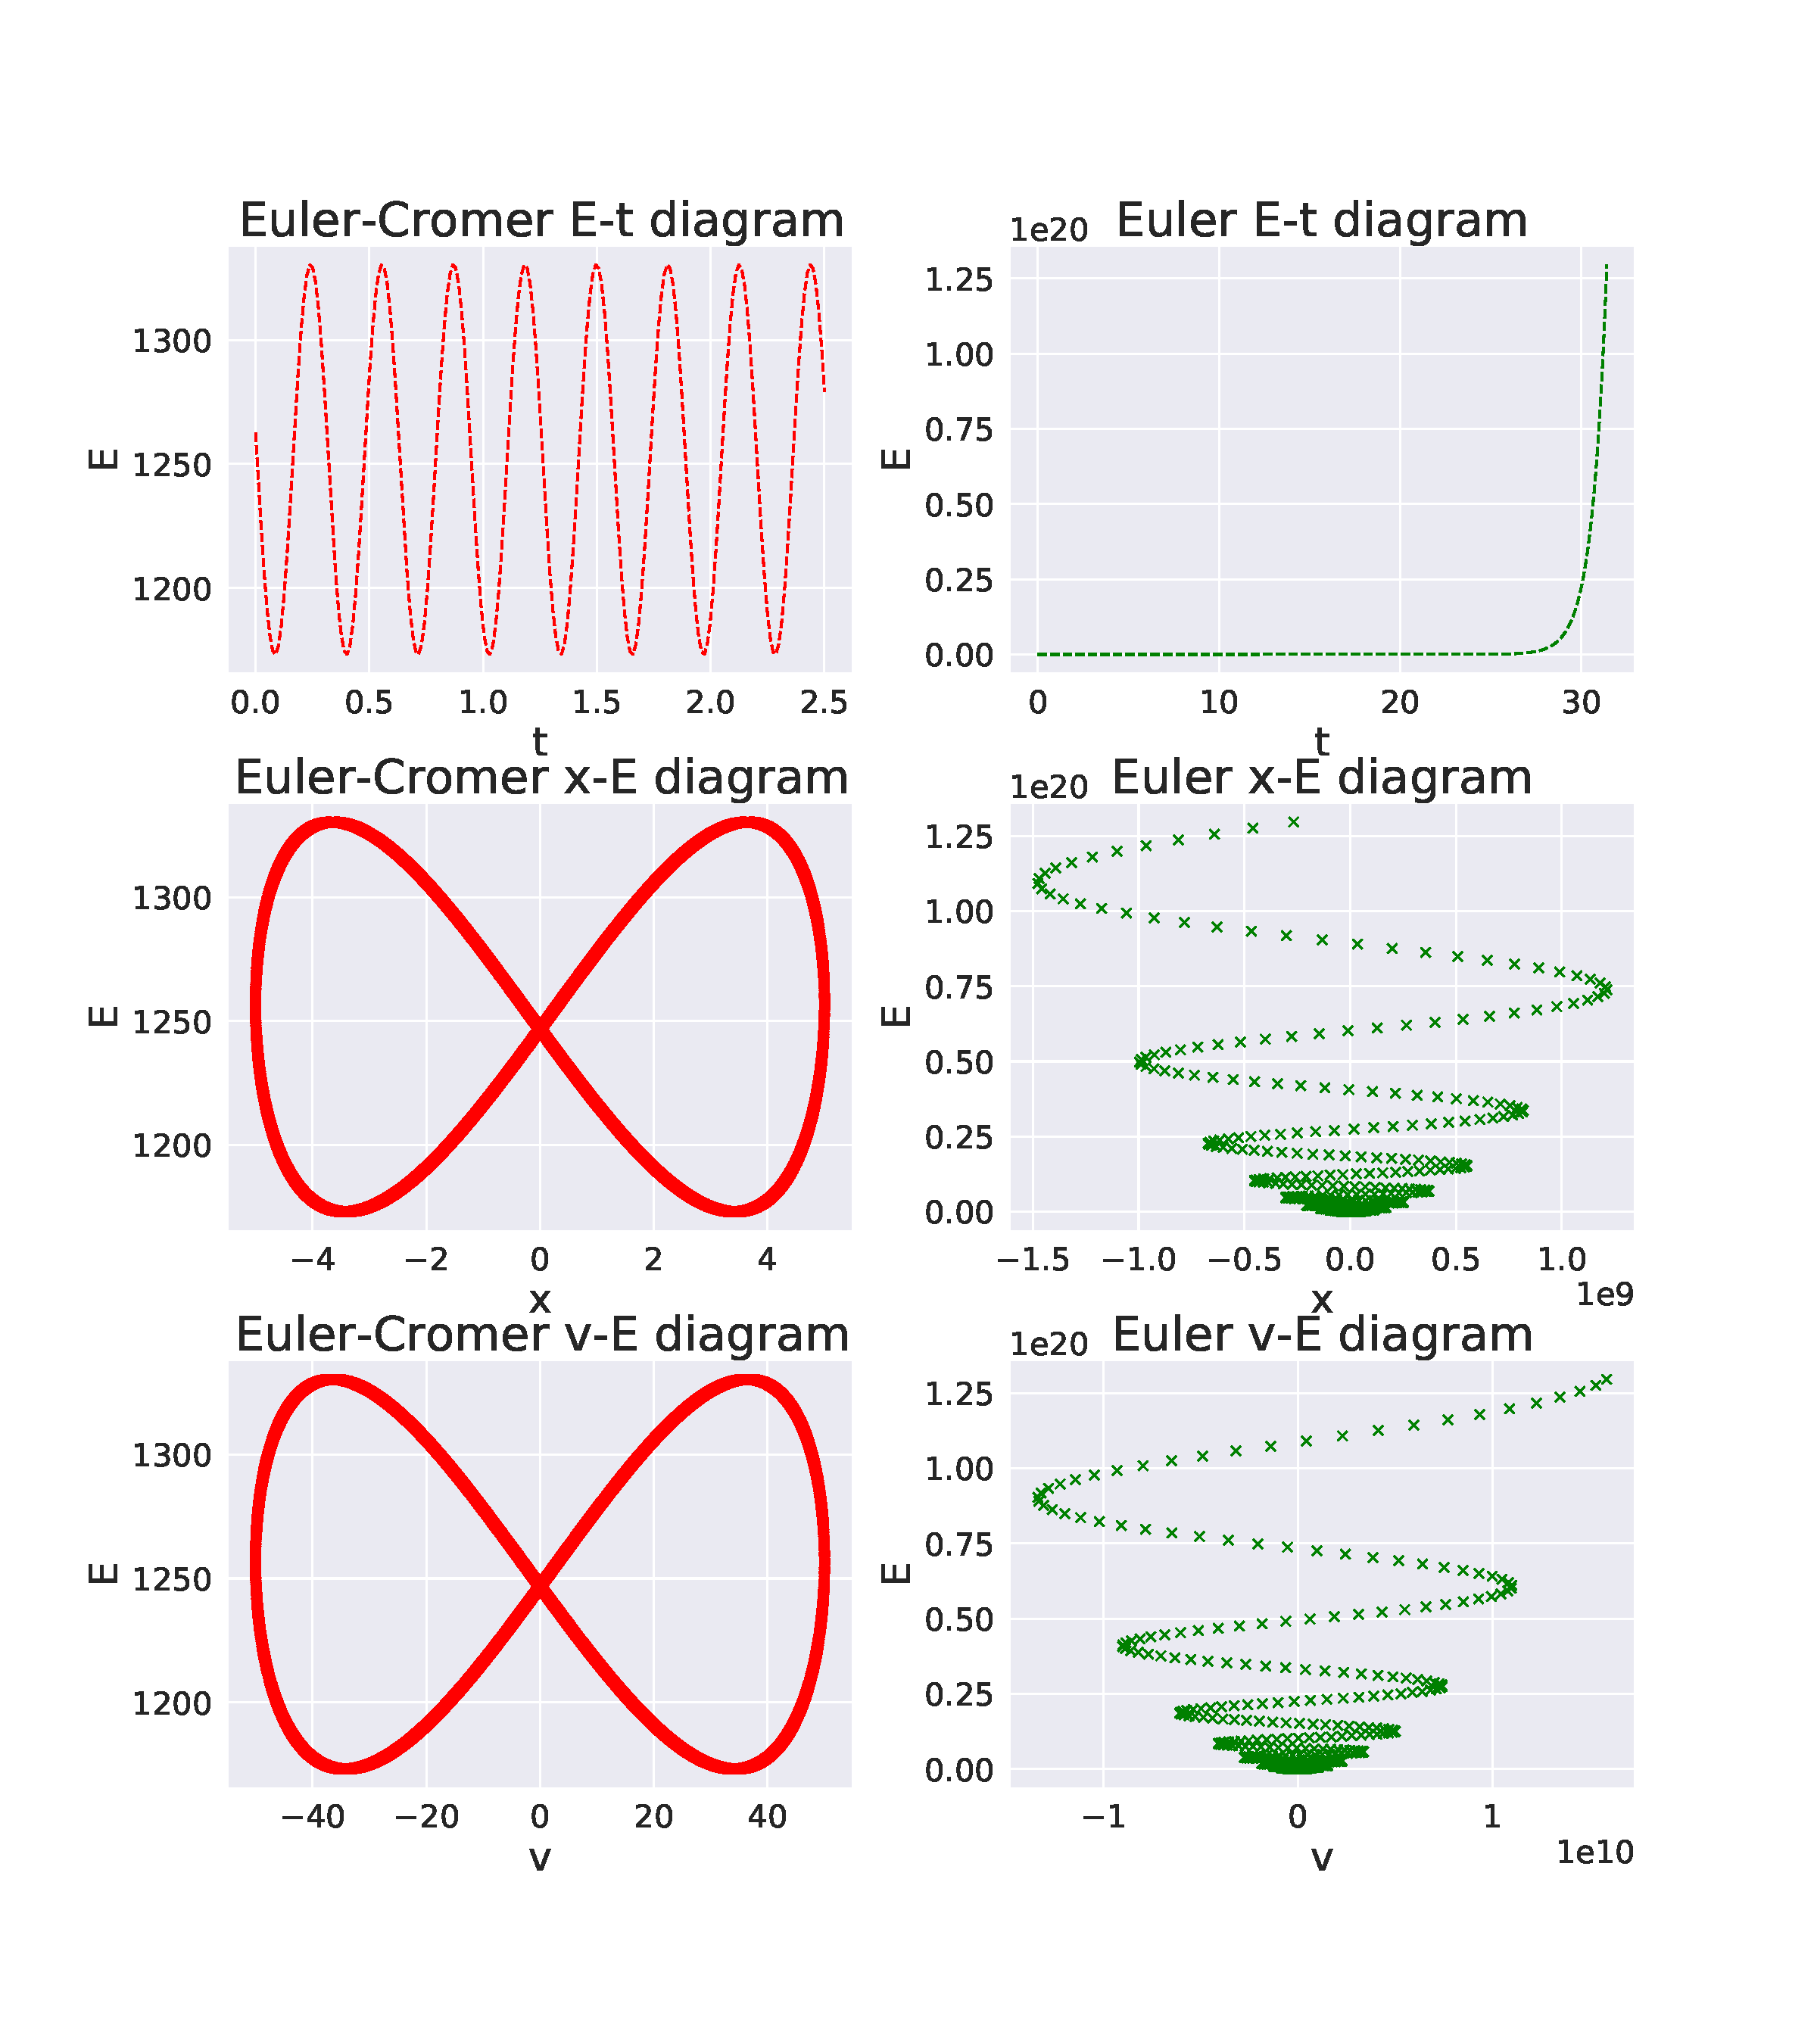
\includegraphics[scale=0.42]{B3.pdf}
\caption{Euler-Cromer és Euler módszer energiaváltozása ($\omega=10$ ; $x_0=5$ ; $v_0=5$ ; periódusok száma=50 ; lépésszám periódusonként=50)}
\end{figure}

Az Euler-Cromer algoritmus energiája periodikusan egy adott tartományban marad, míg az Euler algoritmusé exponenciálisan elszáll.
Az exponenciális változást a kitérés-idő grafikonon is megfigyelhetjük, melyet a következő ábrán szemléltetek, ahol exponenciálist illesztettem a kitérés-idő grafikonra.

\begin{figure}[ht!]
\centering
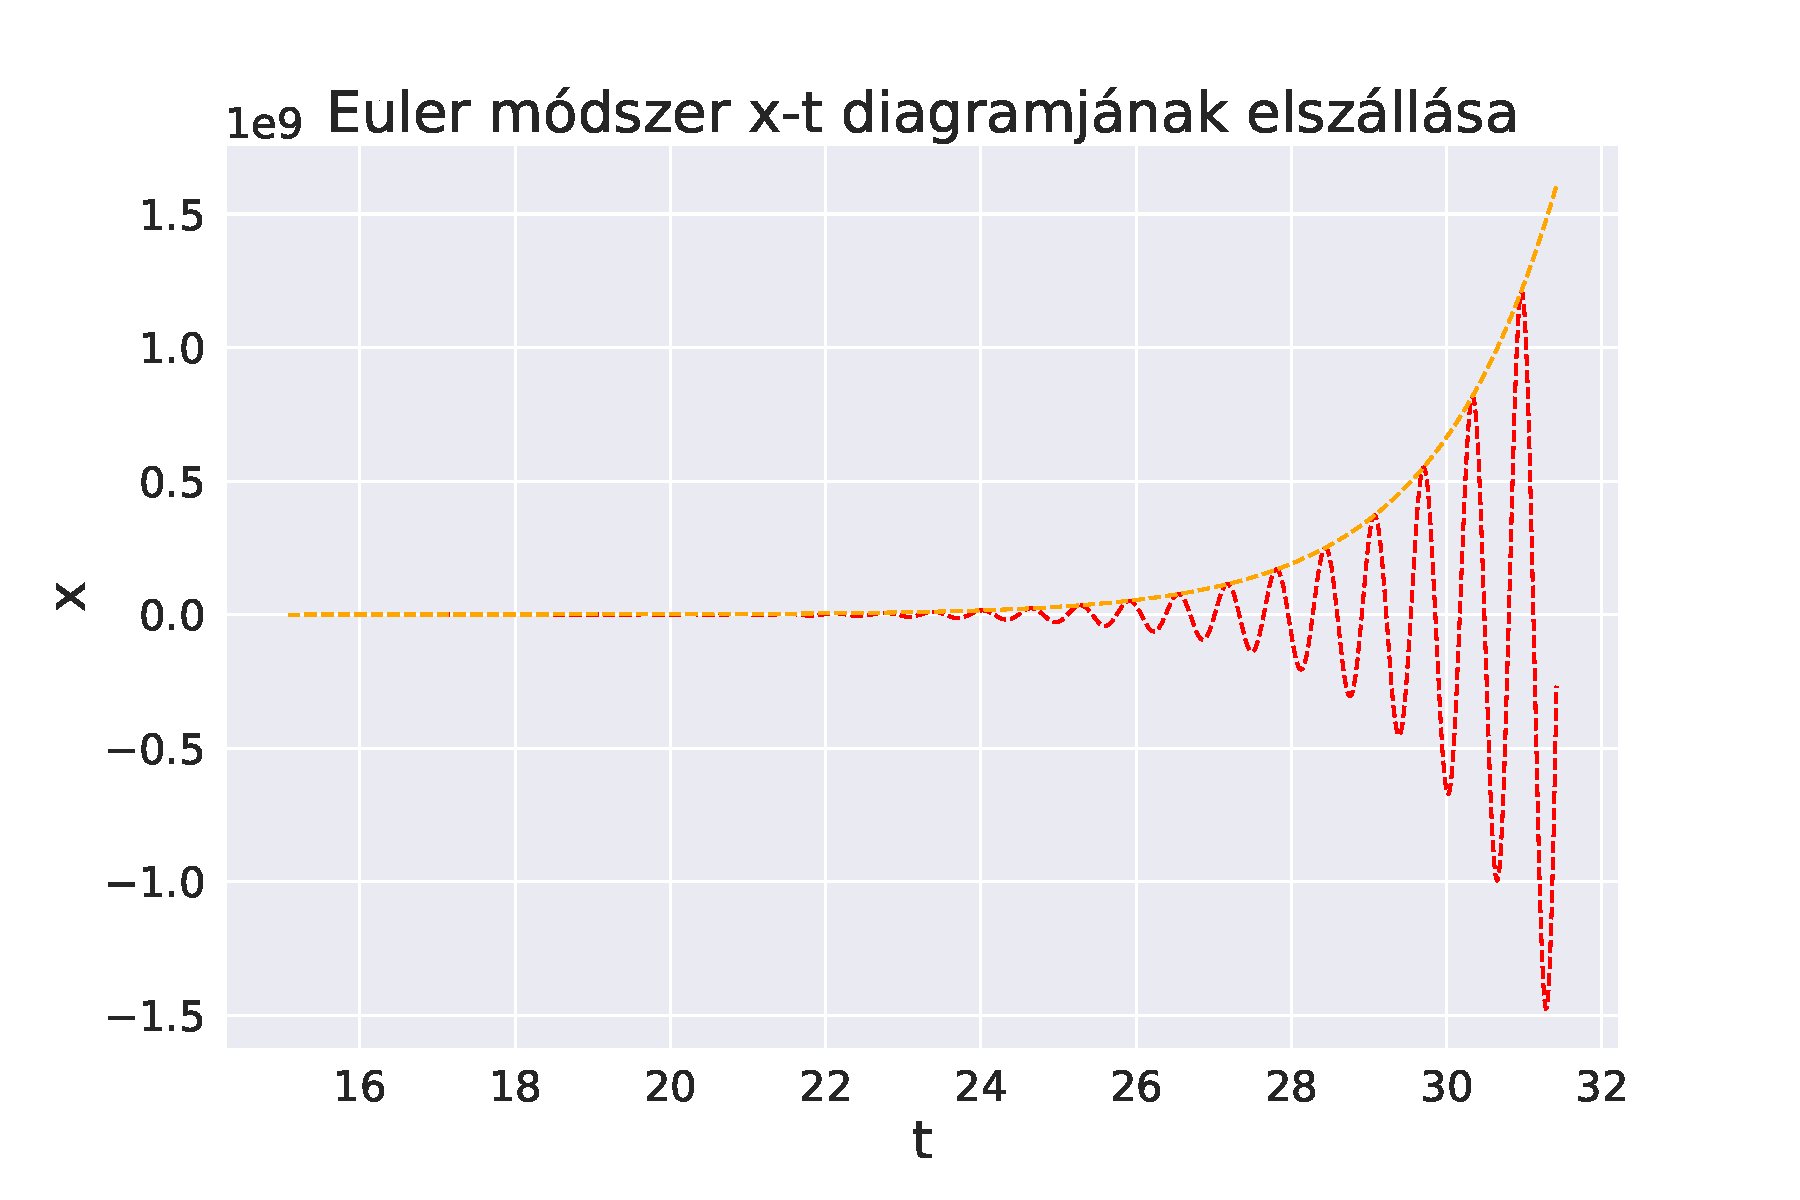
\includegraphics[scale=0.55]{B4.pdf}
\caption{Euler algoritmus kitérésének elszállása az idő függvényében($\omega=10$ ; $x_0=5$ ; $v_0=5$ ; periódusok száma=50 ; lépésszám periódusonként=50)}
\end{figure}

\subsection{Futásidő}

Az utolsó feladat a program futásidejének vizsgálata volt a lépésszámok függvényében. A lépésszámot növelhetjük a periódusonkénti lépésszám növelésével és a periódusok számának növelésével is. Én utóbbi választottam, egy állandó (500 lépés / periódus) számon tartottam a periódusonkénti lépésszámot, és a periódusok számát növeltem lineárisan 50-től 1000-ig 50-esével. A többi paramétert az előző két feladatnak megfelelően vettem fel.

Megvizsgáltam a futásidőt az Euler-Cromer és Euler algoritmus esetén is, ehhez két módosított c++ kódot hoztam létre, melyek külön-külön csak a megadott algoritmus alapján számolnak. A futást ciklusba tettem, amiben az oszcillátor ciklusainak számát növelem. Az egyes ciklusok idejét a chrono könyvtár segítségével mértem meg.

\begin{figure}[ht!]
\centering
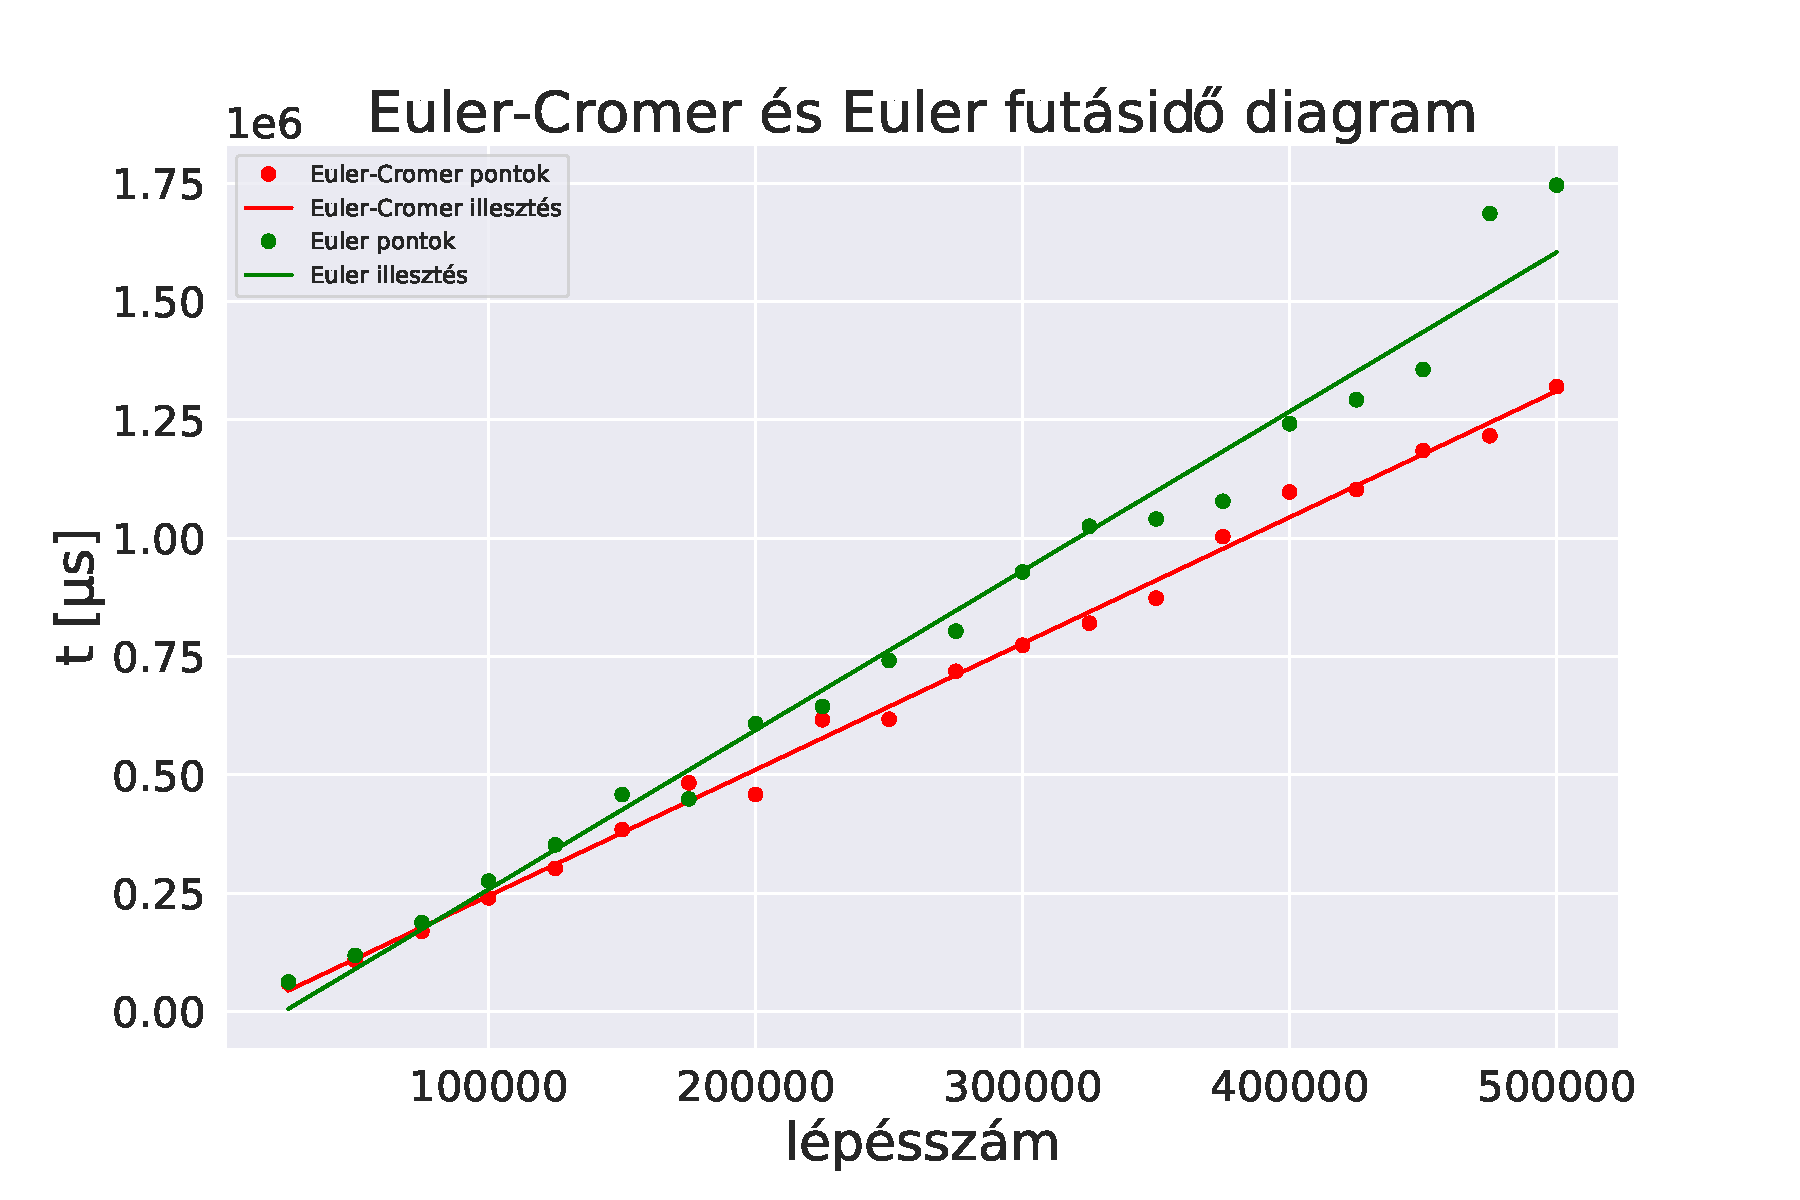
\includegraphics[scale=0.55]{futas.pdf}
\caption{Euler-Cromer és Euler módszer futásidejének vizsgálata ($\omega=10$ ; $x_0=5$ ; $v_0=5$ ; lépésszám periódusonként=500)}
\end{figure}

Az ábra alapján megállapíthatjuk, hogy a futási idő lineárisan nő a lépésszám függvényében az Euler-Cromer és az Euler módszer esetén is, azonban az Euler módszer esetén meredekebb az egyenes, mivel ott a maximum kitérés, a maximum sebesség és az energia értéke is folyamatosan nő (mivel az algoritmus nem stabil), és mivel nagyobb számokkal kell dolgoznia a programnak, a futásidő is hosszabb lesz.

\section{Diszkusszió}

A feladatokat sikeresen elvégeztem, a módosított sho\_m.cpp, sho\_e.cpp, sho\_ec.cpp és a jupyter notebook kódok megtalálhatók a kooplex oldalamon a harmonikus oszcillator mappában.

%\newpage
%\bibliography{ref}
%\newpage
%\appendix
%\renewcommand{\thesection}{\arabic{section}}
%\label{A}
\end{document}
